\section{Terramechanics}
\label{s:Terramechanics}
% -------------------------- paragraph -------------------------------------------------
The tractor-sled vehicle interacts with the terrain at its tracks and at the sled. This section covers the models used for both of these interactions respectively. The modeling techniques for the track forces are from Wong \cite{Wong2008}. Different approaches for modeling the terrain-track interaction exist with varying orders of complexity from empirical, semi-empirical, to complex finite element modeling. In this work, we use semi-empirical Bekker-Wong theory and assume a uniform pressure distribution along the contact length of the track. This theory is well established and provides reasonably accurate predictions for heavy class tracked vehicles. An additive benefit of this approach is that no numerical intergration is required as all expressions are in closed form. This alleviates unnecessary computational load and allows for faster iteration of numerical experiments. A free body diagram of all the track forces is shown in Figure \ref{fig:Free_Body_Diagram_Track}. The driver torque from the output of the powertrain $\tau$, the traction force, $F$, and compaction resistance, $R_c$, are denoted as blue arrows. The lateral resistance forces, $R_l$, are shown as green arrows. All of these forces are functions of slip, vehicle parameters, and terrain parameters. 
The traction, compaction resistance and sinkage for a single track are given by
\begin{linenomath*}
    \begin{equation} \label{eq:tractionForce}
        F = (Ac + W\tan\Phi) \Big(1 - \frac{K}{il} \Big(1 - e^{\frac{il}{K}}\Big) \Big)
    \end{equation}
\end{linenomath*}
\begin{linenomath*}
    \begin{equation} \label{eq:compactionResistance}
        R_c = b\bigg(\frac{k_c}{b} + k_\Phi\bigg)\frac{z^{n+1}}{n+1}
        %R_c = \frac{bl}{(n+1)(k_c/b + k_{\Phi})^{1/n}} \Big( \frac{W}{bl} \Big)^{n + 1/n}
    \end{equation}
\end{linenomath*}
\begin{linenomath*}
    \begin{equation} \label{eq:sinkage}
        z = \bigg(\frac{W/A}{(k_c/b) + k_\Phi}\bigg)^{1/n}
        %p = \Big(\frac{k_c}{b} + k_{\Phi}\Big)z^n 
    \end{equation}
\end{linenomath*}
%\begin{linenomath*}
%    \begin{equation}
%        R_b = b(0.67czK_{pc} + 0.5z^2\gamma_s K_{p\gamma})
%    \end{equation}
%\end{linenomath*}
\begin{figure}[tb]
    \centering
    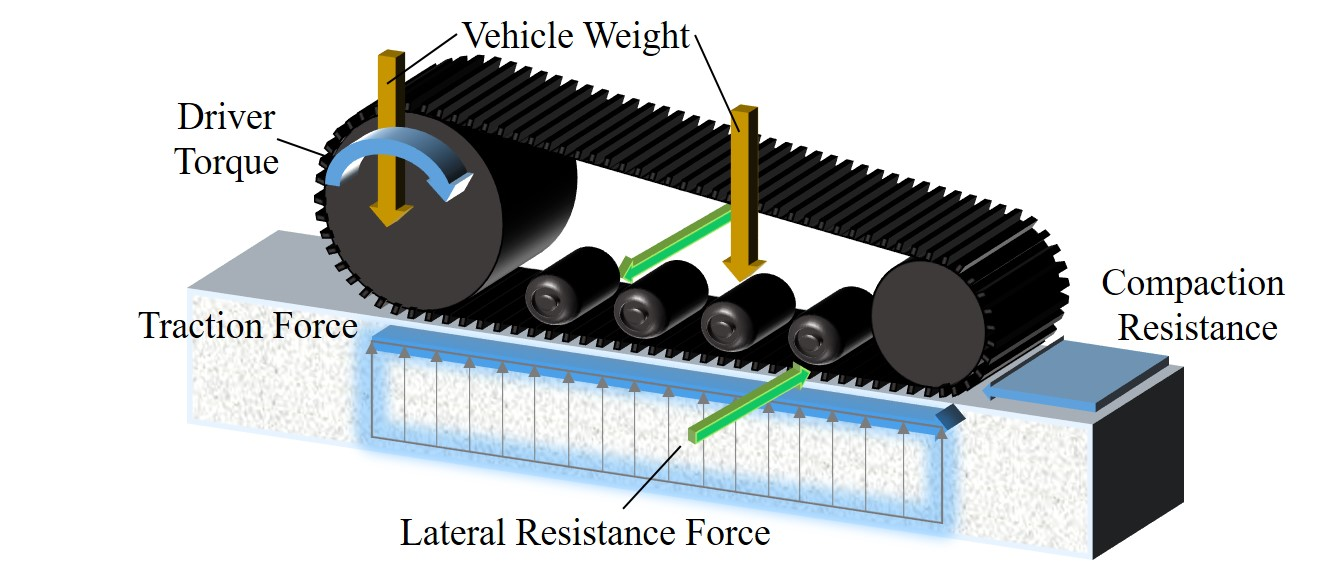
\includegraphics[width=5.5in]{Free_Body_Diagram_Track}
    \caption{Track Free Body Diagram}
    \label{fig:Free_Body_Diagram_Track}
\end{figure}
where $A$ is the nominal ground contact area of one track, $c$ is the terrain cohesion, $W$ is the normal load for one track on the terrain, $\Phi$ is the terrain friction angle, $K$ is the terrain shear deformation modulus, $i$  is the slip ratio, $k_c$ is the cohesive modulus of terrain deformation, $k_\Phi$ is the friction modulus of terrain deformation, $n$ is the exponent of terrain deformation, and $z$ is the sinkage. Equations \ref{eq:tractionForce}, \ref{eq:compactionResistance} and \ref{eq:sinkage} summarize Bekker-Wong terramechanics theory and dictate the longitudinal motion of the vehicle \cite{Wong2008}.
% ------------------------------------------- paragraph -------------------------------------------------

As a vehicle attempts to turn however, additional lateral resistive forces act on the vehicle tracks. There is no well established method for determining these forces based on Bekker-Wong terrain parameters. However, experimental data shows that these forces depend on the normal load on the terrain, the vehicle turning radius, and vehicle speed \cite{Wong2008}. Since SPT uses agricultural tractors, we omit any dependence on speed since there is a limited operating range approximately between $0$ - $4$ $m/s$. The equation for each of the lateral resistance forces is given by
\begin{linenomath*}
    \begin{equation}
        R_l = -sign(v_{y,track})(\mu_r(\rho) + \mu_z(z))W
    \end{equation}
\end{linenomath*}
where $v_{y,track}$ is the velocity of the track segment in the $\mathbf{j}_1$ direction, $\mu_r$ is the lateral resistance coefficient based on the turning radius, $\rho$, and $\mu_z$  is the coefficient of lateral turning resistance based on the sinkage at the given track segment. To calculate $\mu_r$, a log linear approximation is made based on data trends provided in \cite{Wong2008} and is given by
\begin{linenomath*}
    \begin{equation}
        \mu_r = -m_{\rho}\log(\rho) + h_{\rho}
    \end{equation}
\end{linenomath*}
where $m_\rho$ and $h_\rho$ are the coefficients for the slope and offset. There is not an established method for calculating the lateral resistance coefficient due to sinkage $\mu_z$ but it is postulated that it does have a notable impact on the vehicle's trajectory and is a function of existing terrain parameters. Therefore, this is left as an input to the model. 
% ------------------------------------------- paragraph -------------------------------------------------

The model for the sled friction forces is derived from data and methods in Lever and Weale \cite{lever2012high}. The data provided measures the drawbar pull directly at the tractor hitch. The figure from the study and instrumentation used to collect it are shown in Fig. \ref{fig:Sled_Data}. It is assumed that since the tractor accelerates slowly, that the measured drawbar value is approximately equal to the sled resistance coefficient, $\eta$ at the sled-snow interface. Furthermore, other data from \cite{lever2012high} shows resistance coefficents to be as low as $0.03$. This data is used to empirically model the frictional force at the sled snow interface, $R_{SD}$ using the resistance coefficient $\eta$ bounded between 0.03 to 0.13.
\begin{figure}[htb]
\begin{subfigure}{0.6\textwidth}
\centering
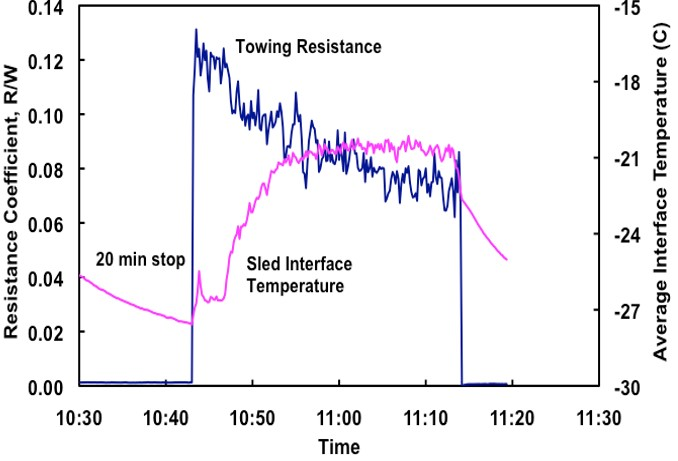
\includegraphics[height = 5cm, keepaspectratio]{Sled_Transient_Coeff_Plot} 
\caption{}
\label{fig:Sled_Transient_Coeff_Plot}
\end{subfigure}
\begin{subfigure}{0.5\textwidth}
\centering
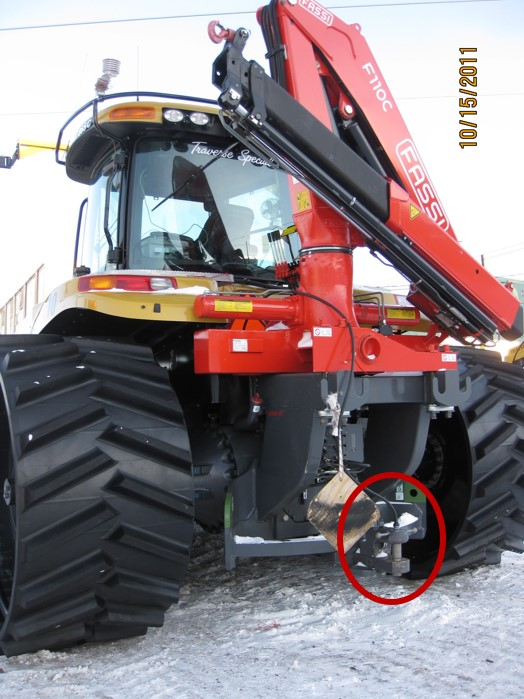
\includegraphics[height = 5cm, keepaspectratio]{Tractor_Load_Pin}
\caption{}
\label{fig:Tractor_Load_Pin}
\end{subfigure}
\caption{(a) Plot of polar sled transient resistance coefficient vs time and temperature. Reproduced from \cite{lever2012high}. (b) Rear View of an AGCO MT865 tractor. The load pin used to collect data is circled in red. Photo Credit: James H. Lever}
\label{fig:Sled_Data}
\end{figure}
\begin{linenomath*}
    \begin{equation} \label{eq:resistanceSled}
        R_{SD} = \eta m_B g N
    \end{equation}
\end{linenomath*} 
It is postulated that $\eta$ also depends on the terrain and operating speed of the tractor but no data is available yet to show this relationship. For the single body dynamics model, it is assumed the $R_{SD} = DB$ where $DB$ is the drawbar load at the tractor's hitch.